\section{Begriffe}

\subsection{Objekt \balzert{20}}
	Ein Objekt wird aus einer Klasse erzeugt, ist also ein Exemplar einer Klasse. Generell
	ist ein Objekt ein Gegenstand des Interesses, eine Beobachtung usw. Oft wird als
	Synonym auch Instanz verwendet.
	\begin{description}
		\item[Zustand] Der Zustand umfasst die Attribute, ihre aktuellen Werte, sowie
			die Objektbeziehungen (\textit{links}).
		\item[Verhalten] Das Verhalten wird durch die Operationen beschrieben. Eine
			Änderung des Zustands ist nur durch Operationen möglich.
		\item[Objektidentität] jedes Objekt hat eine Identität, welche einzigartig ist
			(unique)
	\end{description}
	\subsubsection{Notation}
		Objektnamen werden immer klein geschrieben und unterstrichen. \\
		\begin{tabular}{l l}
			\underline{:Klasse} & anonymes Objekt \\
			\underline{objekt:Klasse} & Objekt wird über Namen angesprochen \\
			\underline{objekt} & wenn Objektname zur Identifikation ausreicht \\
		\end{tabular}\\
	\begin{multicols}{2}	
	\subsubsection{Geheimnisprinzip}
	Daten sind nach aussen verborgen und können nur über Operationen gelesen oder geändert werden.\\
	\subsubsection{Objektidentität}
	Eigenschaft, die ein Objekt von allen anderen Objekten unterscheidet. Bei zwei Objekten
	mit gleichen Attributwerten sprechen wir von Gleichheit, wenn dasselbe Objekt gemeint
	ist von Identität.
	\end{multicols}
	
	\subsection{Klasse \balzert{23}}
	Eine Klasse ist eine Vorlage für ein Objekt. \\
	\begin{minipage}[t]{4cm}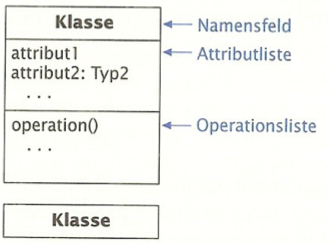
\includegraphics[width=4cm]{./images/klasse.png}\end{minipage}
	\begin{minipage}[c]{16cm}
		\begin{description}
		\item[Attribut] Beschreibt Daten die von den Objekten der Klasse angenommen
			werden können. Alle Objekte einer Klasse haben dieselben Attribute, können
			aber unterschiedliche Attributwerte haben.
		\item[Klassenattribut] wenn nur ein Attributwert für alle Objekte einer Klasse
			existiert. Sie existieren auch, wenn es zu einer Klasse noch keine Objekte
			gibt.
		\item[Operation] Eine Funktion die auf alle Attributwere eines Objekts Zugriff
			hat.
		\item[Klassenoperation] Eine Operation, die der jeweiligen Klasse zugeordnet
			ist kann nicht auf ein einzelnes Objekt der Klasse angewendet werden. 
		\item[Verhalten] Das Verhlaten der Klasse ist die Menge aller Operationen
		\item[Abstrakte] Von einer abstrakten Klasse können keine Objekte erzeugt
			werden. Abstrakte Klassen werden durch kursiven Klassennamen oder mittels
			\{abstract\} gekennzeichnet.
		\item[Basisklasse] Vererbt abgeleiteten Klassen Attribute und Operationen
		\end{description}
	\end{minipage}
	\subsubsection{Notation}
		Der \textbf{Klassenname} ist immer ein Substantiv im Singular, das durch ein Adjektiv
		ergänzt werden kann. Der Klassenname wird fett geschrieben und beginnt mit einem
		Grossbuchstaben. \\
		
	
\subsection{Komponente}
	Ist ein Softwarebaustein, der über klar definierte Schnittstellen Verhalten
	(Funktionalität) bereitstellt.
	interface
	component

\subsection{Assoziation}
	Modelliert Objektbeziehungen zwischen Objekten einer oder mehrerer Klassen.
	Jede Assoziation wird durch Mutliplizitäten, einen optionalen Namen oder Rollennamen
	beschrieben.
\begin{description}
	\item[binäre Assoziation] Assoziation zwischen 2 Objekten
	\item[ternäre Assoziation] Assoziation zwischen 3 Objekten
	\item[n-äre Assoziation] zwischen n Objekten
	\item[reflexive Assoziation] Verbindet zwei Objekte der gleichen Klasse
	\item[Assoziationsklasse] Besitzt die Eigenschaften einer Assoziation und einer
		Klasse
	\item[Aggregation] Sonderfall der Assoziation. "`ist Teilvon"' oder "`besteht
		aus"'.
	\item[Komposition] besondere Form der Aggregation. Beim löschen müssen auch
		alle Teile gelöscht werden. Jedes Teil kann nur zu einem Ganzen gehören 
	\item[Navigationsrichtung] Das erzeugen des einen erzwingt die Erzeugung des
		Anderen
	\item[Multiplizität] Bezeichnet die Wichtigkeit derAssoziation. Bezeichnet die
		Anzahl der an der Assoziation beteiligten Objekte.
	\item[abgeleitete Assoziation] Die Abhängigkeiten sind bereits durch andere
		Assoziationen beschrieben worden.
	\item[Assoziationsname] Beschreibt im Allgemeinen nur eine Richtung der
		Assoziation. Kann fehlen wenn captian obvious unterwegs ist.
	\item[Leserichtung] Angabe beim Assoziationsnamen
	\item[Sichtbarkeit] Vor dem Rollenname geschriben. -private \#protected +public
		$\sim$package
	\item[Eigenschaftswert] Kann bei Bedarf an das Assoziationsende geschrieben
		werden. (z.B.: Ordnend)
	\item[Rollenname] Bei der Klasse, deren Bedeutung sie beschreibt. Kann zur
		Verständlichkeit beitragen.
\end{description}

\subsection{Generalisierung}
Beschreibt die Beziehung zwischen einer allgemeinen Klasse (Basisklasse) und
einer spezialisierten Klasse. Die spezialisierte Klasse ist vollständig
konstistent mit der Basisklasse, enthält aber zusätzliche Informationen
(Attribute, Operationen, Assoziationen).
	\begin{description}
		\item[Vererbung] Unterklasse kann alle eigenschaften als Oberklasse
		mitbenutzen
		\item[Einfachvererbung]
		\item[Mehrfachvererbung]
		\item[Generalisierung] Die spezialisierte Klasse erweitert die Liste der
		Attribute, Operationen und Assoziationen der Basisklasse
		\item[Generalisierungsmenge] spezifiziert, nach welchen Kriterien eine
		Generalisierung modelliert wird
	\end{description}
	
